
\begin{figure}[H]
    \centering
    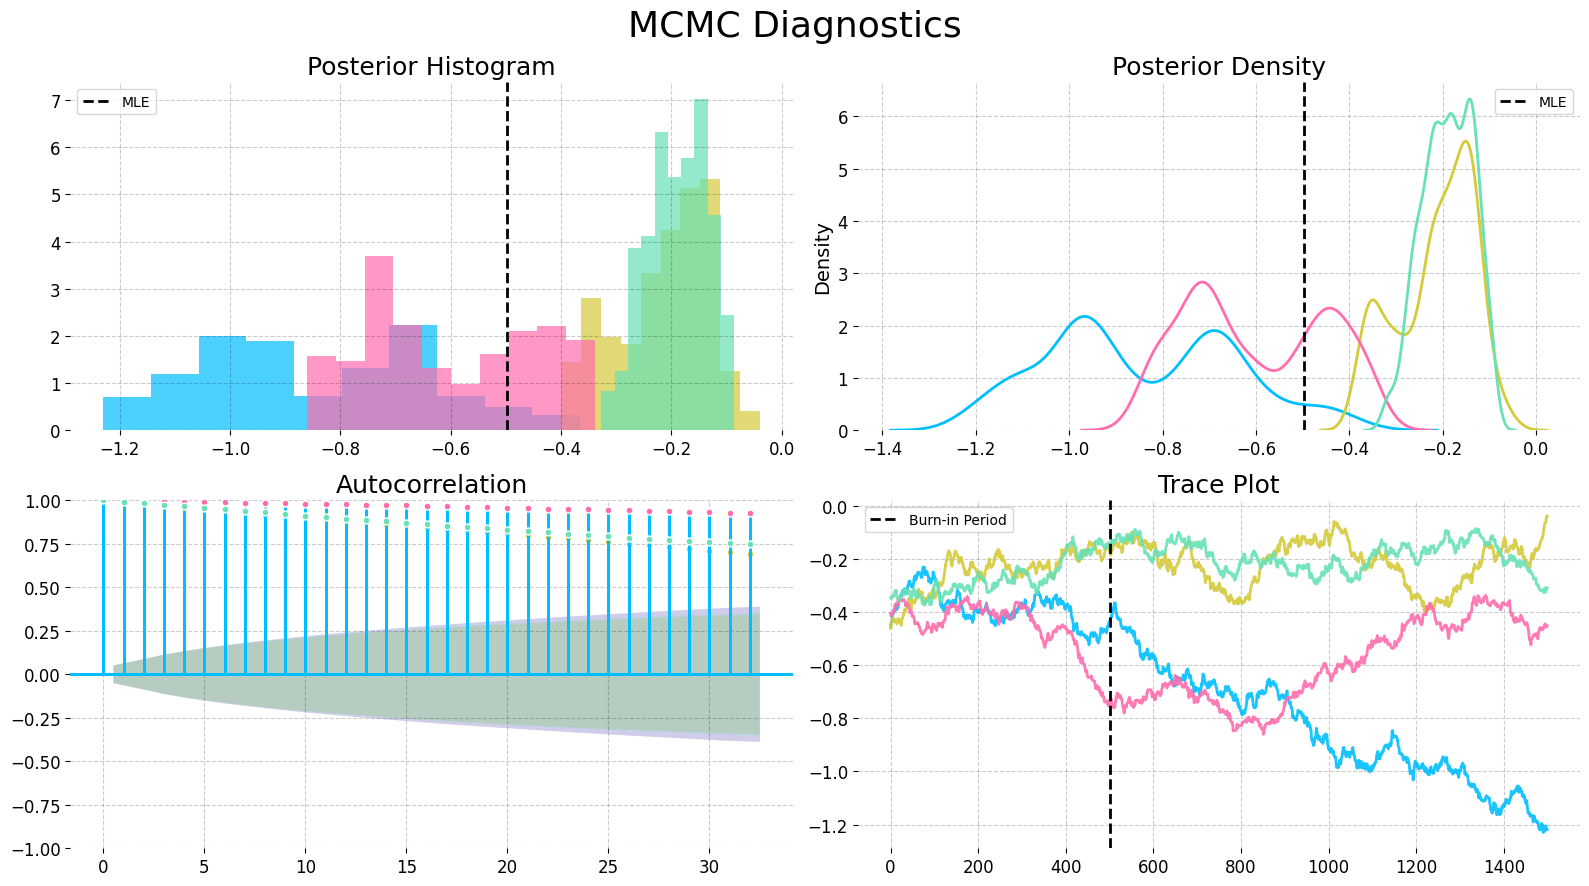
\includegraphics[width=\textwidth/\real{1.25}]{imgs/pmcmc/mh.png}
    \caption{Convergence diagnostics for the Metropolis-Hastings variant particle MCMC with the random walk proposal and an informative empirical prior from IF2. Here, we display the results for the trend parameter in the Dhaka cholera model of \cite{king08}.}
    \label{fig:mh}
\end{figure}


\begin{figure}[H]
    \centering
    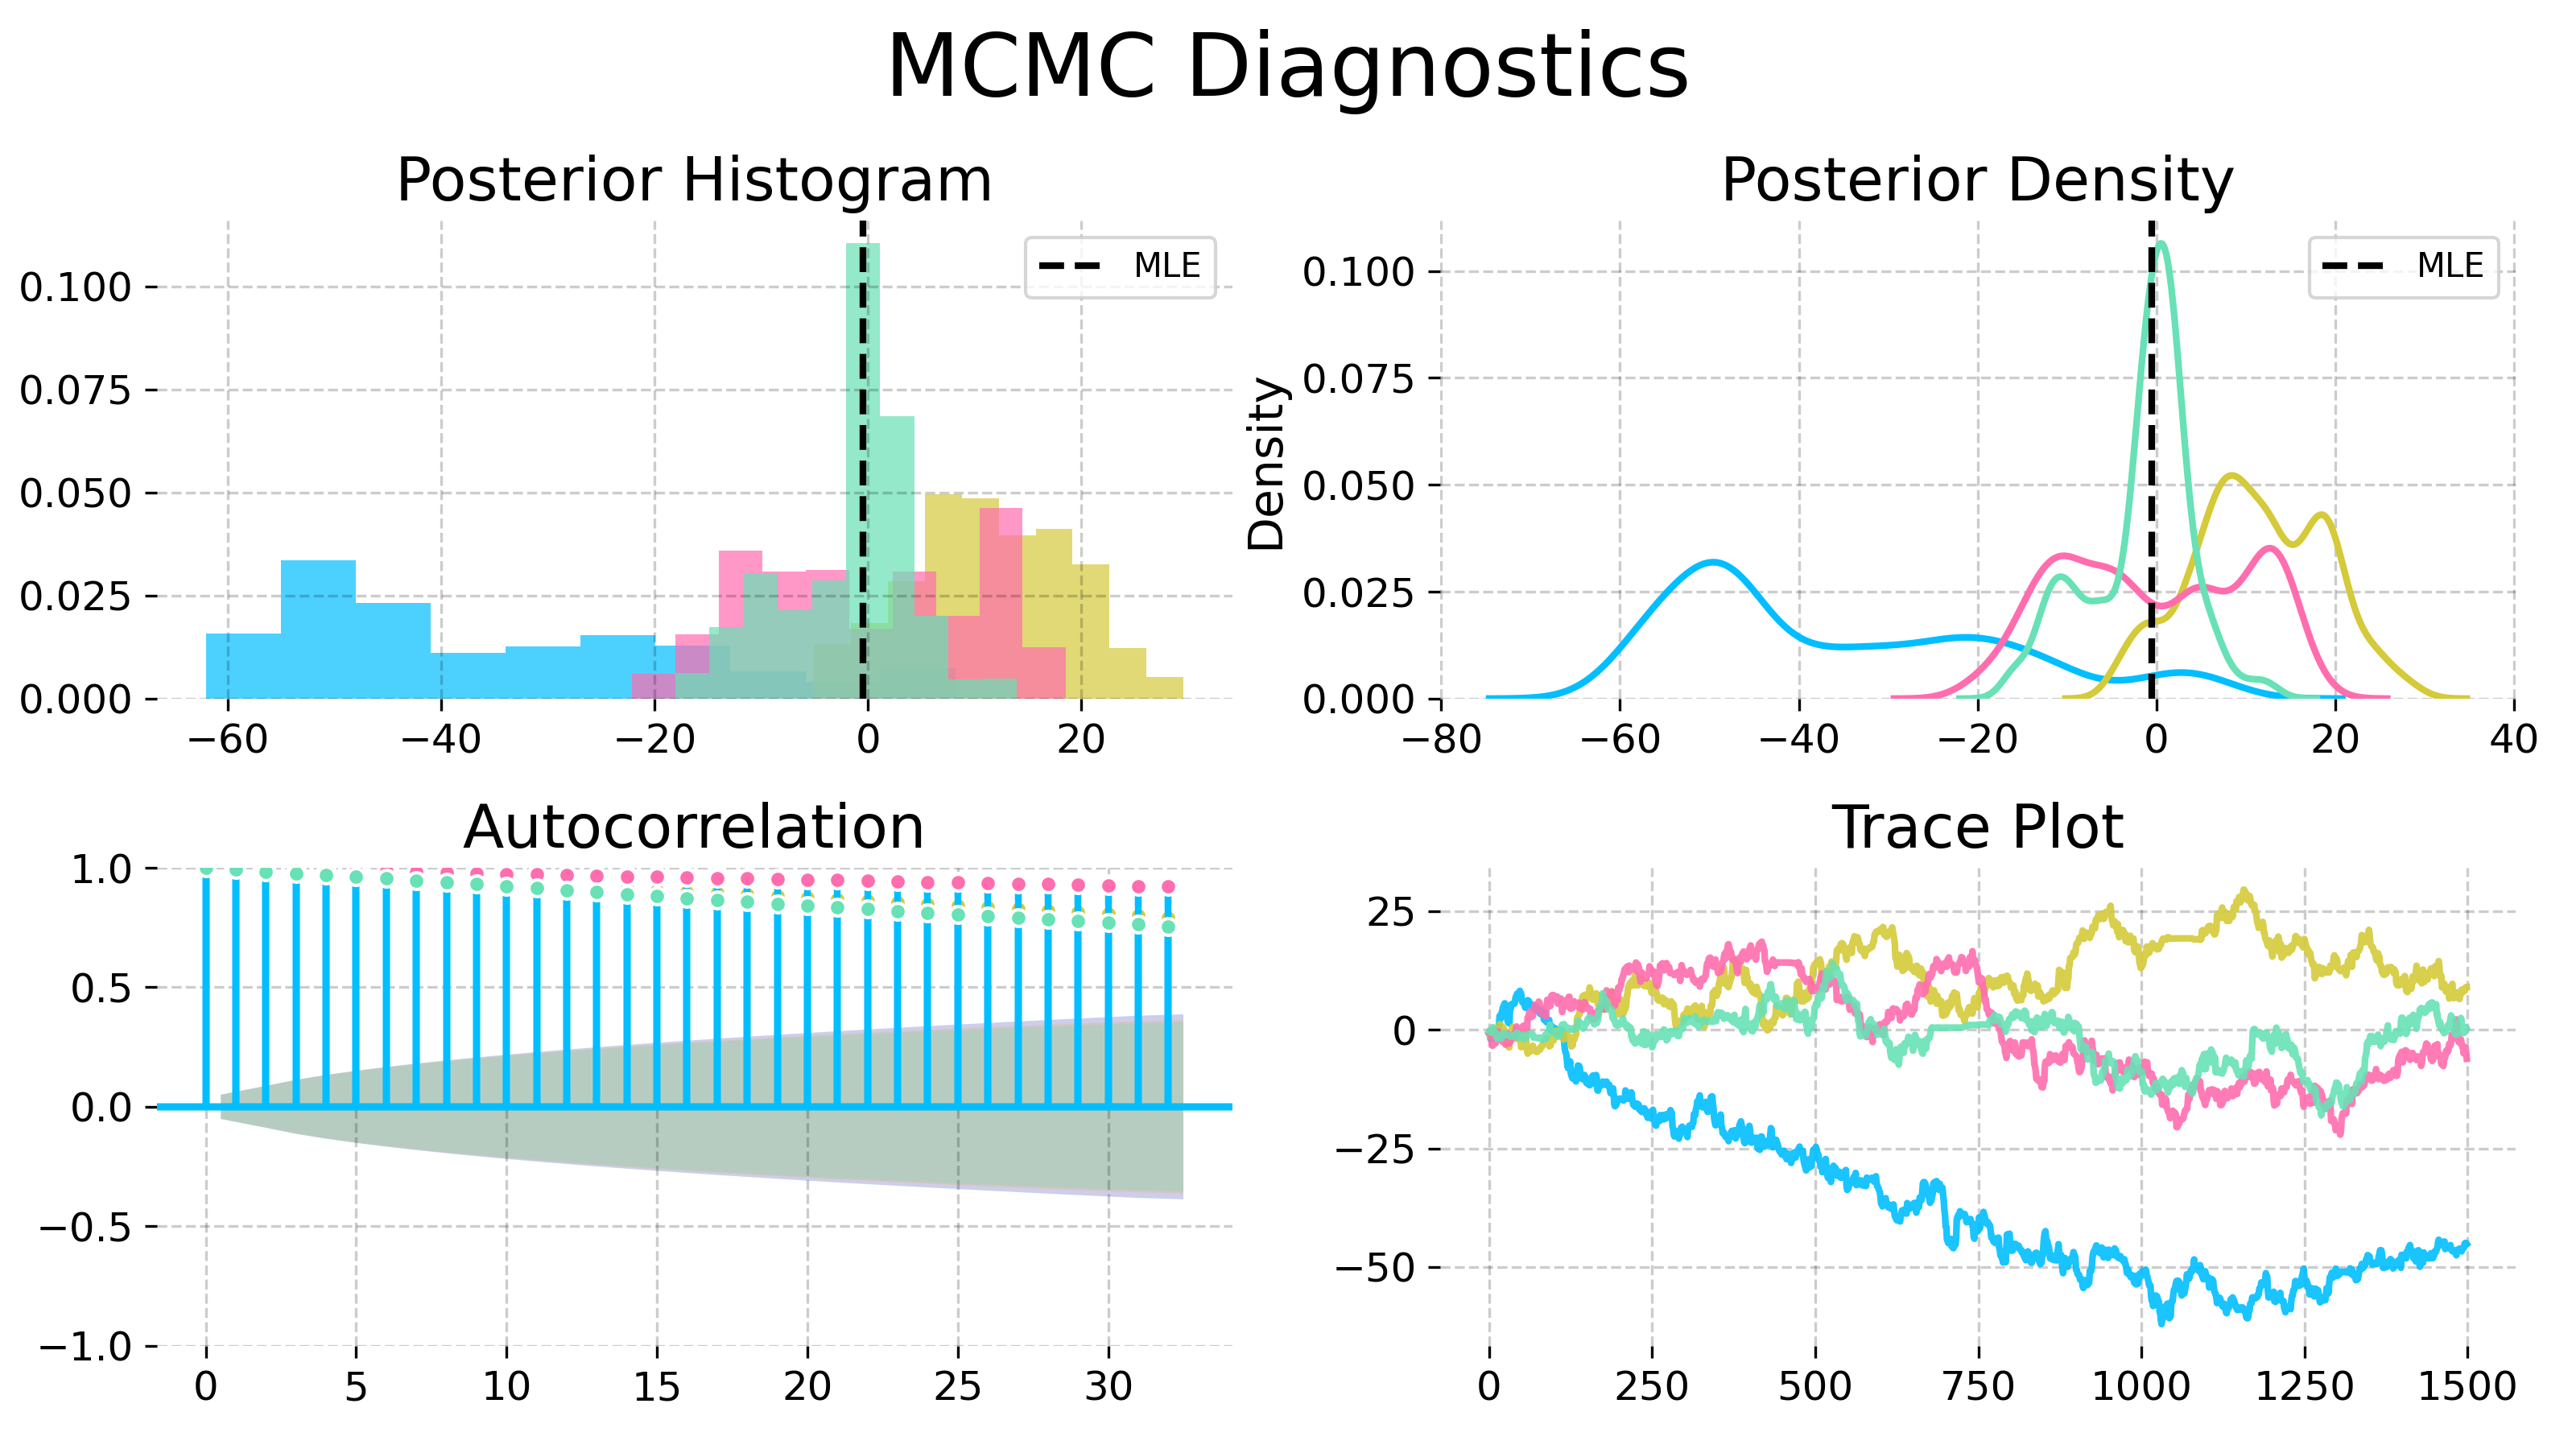
\includegraphics[width=\textwidth/\real{1.25}]{imgs/pmcmc/nuts.png}
    \caption{Convergence diagnostics for a No U-Turn Sampler with uniform priors on a compact set. Again, we display the results for the trend parameter in the Dhaka cholera model of \cite{king08}. The NUTS sampler explores more of the posterior than the MH sampler, but fails to converge quickly.}
    \label{fig:nuts}
\end{figure}


\begin{figure}[H]
    \centering
    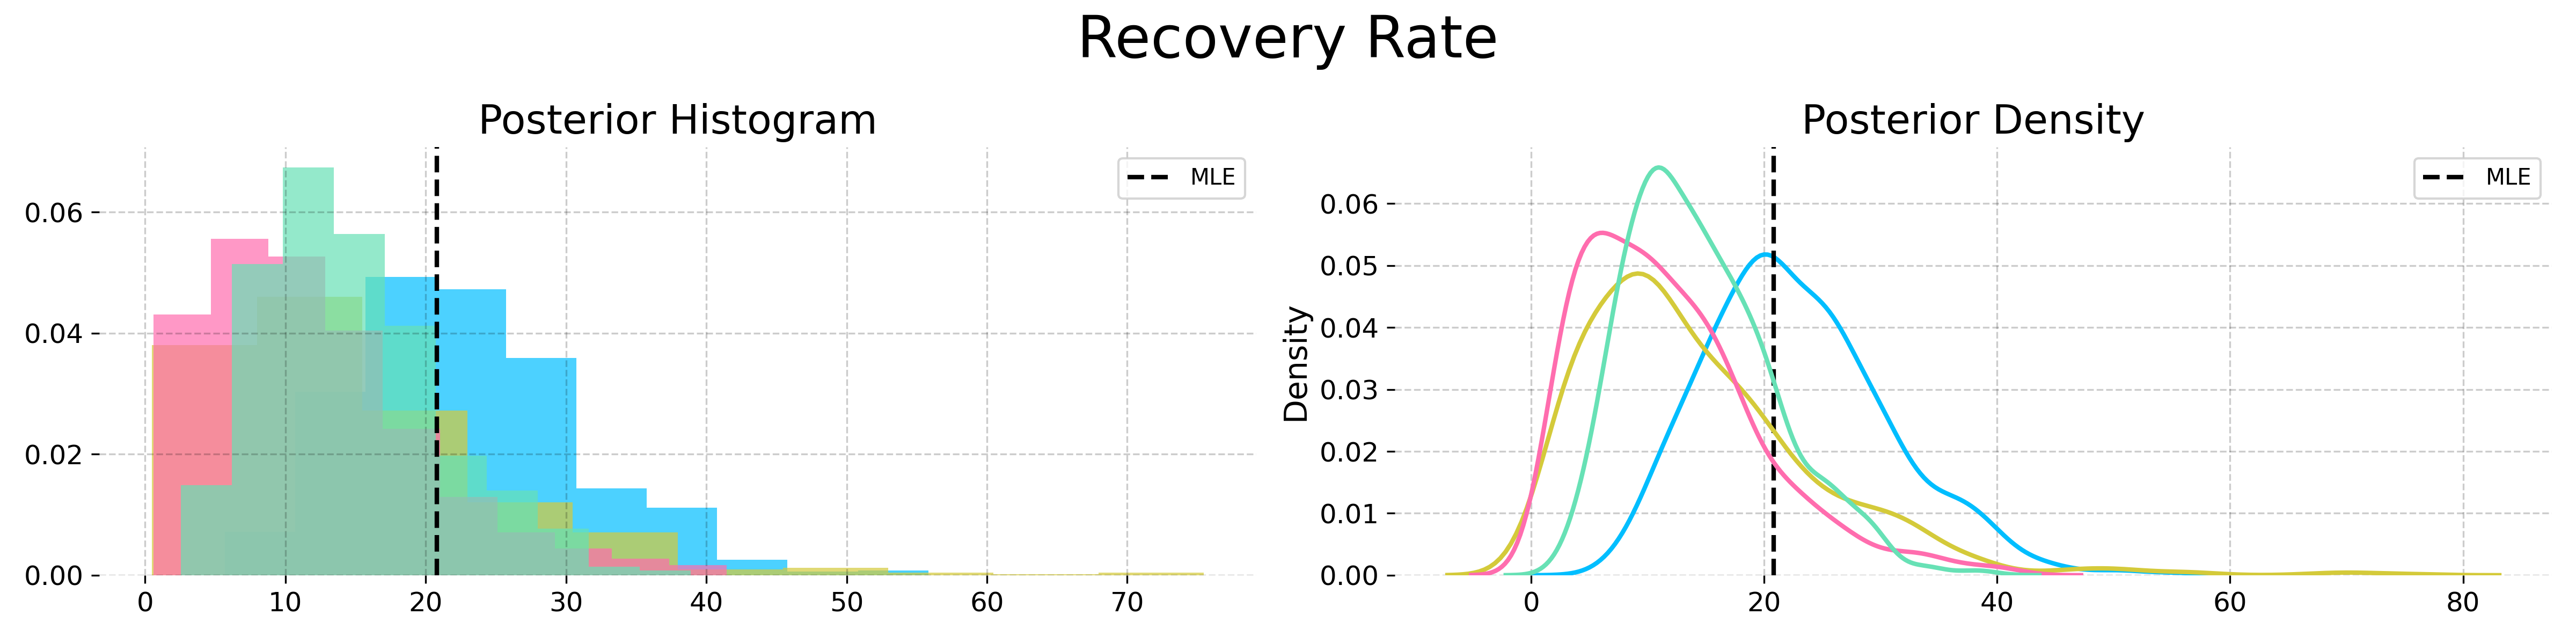
\includegraphics[scale=0.3]{imgs/pmcmc/nuts_eb/Recovery Rate.png}
    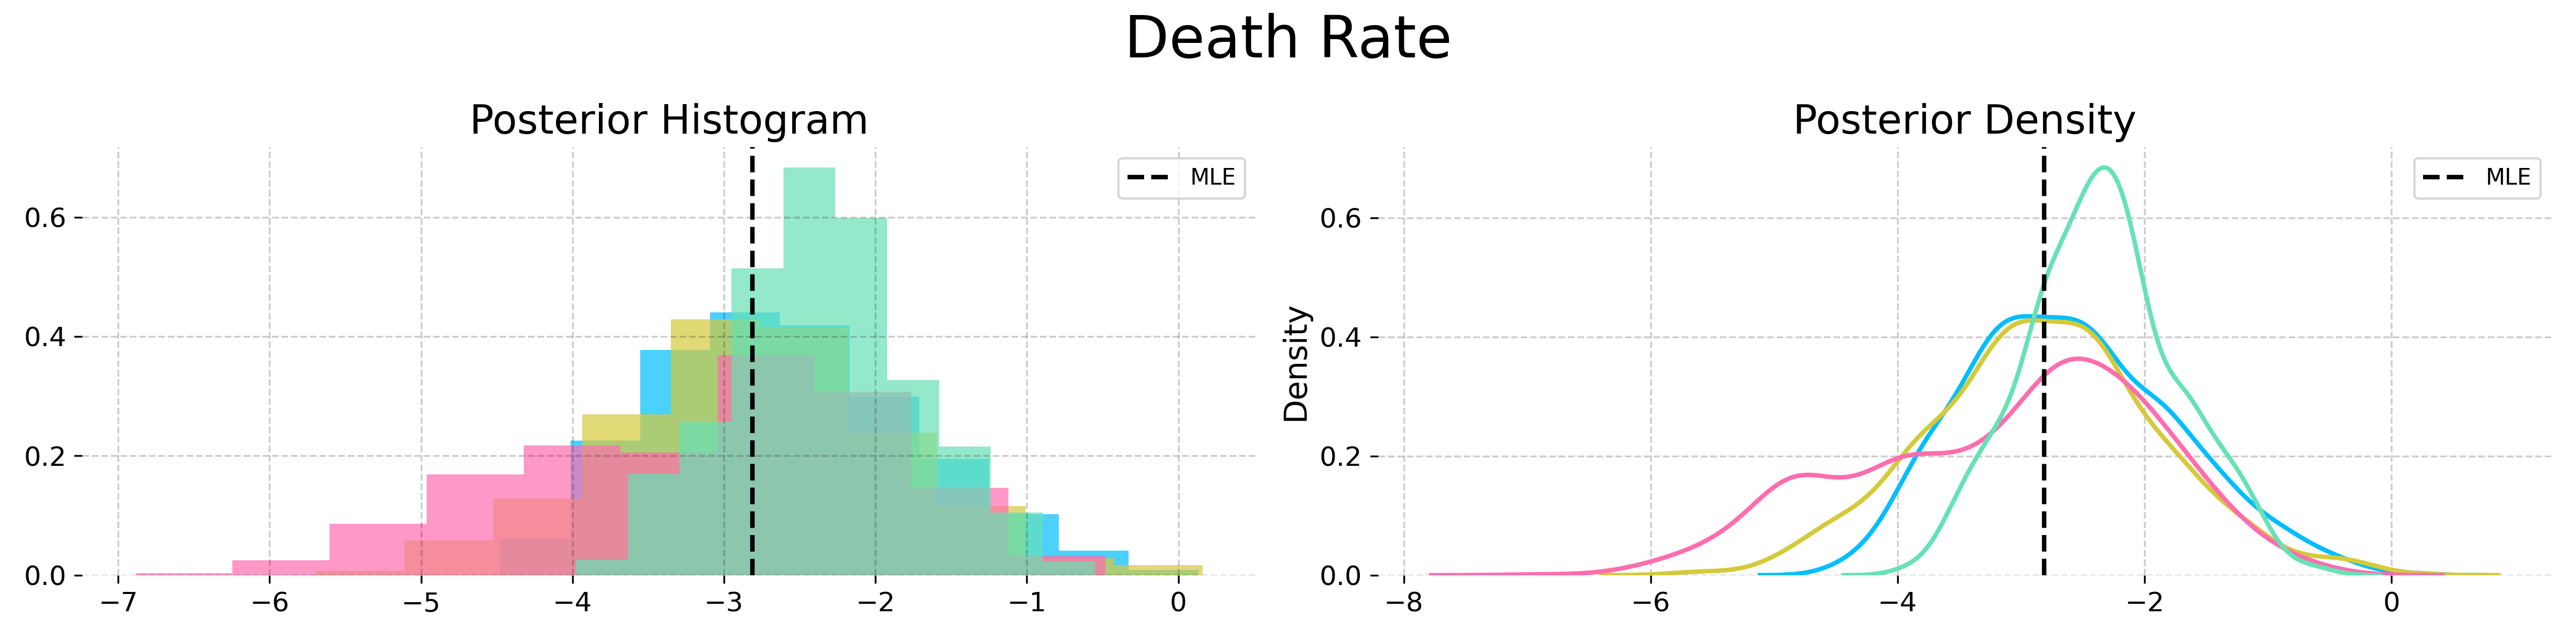
\includegraphics[scale=0.3]{imgs/pmcmc/nuts_eb/Death Rate.png}
    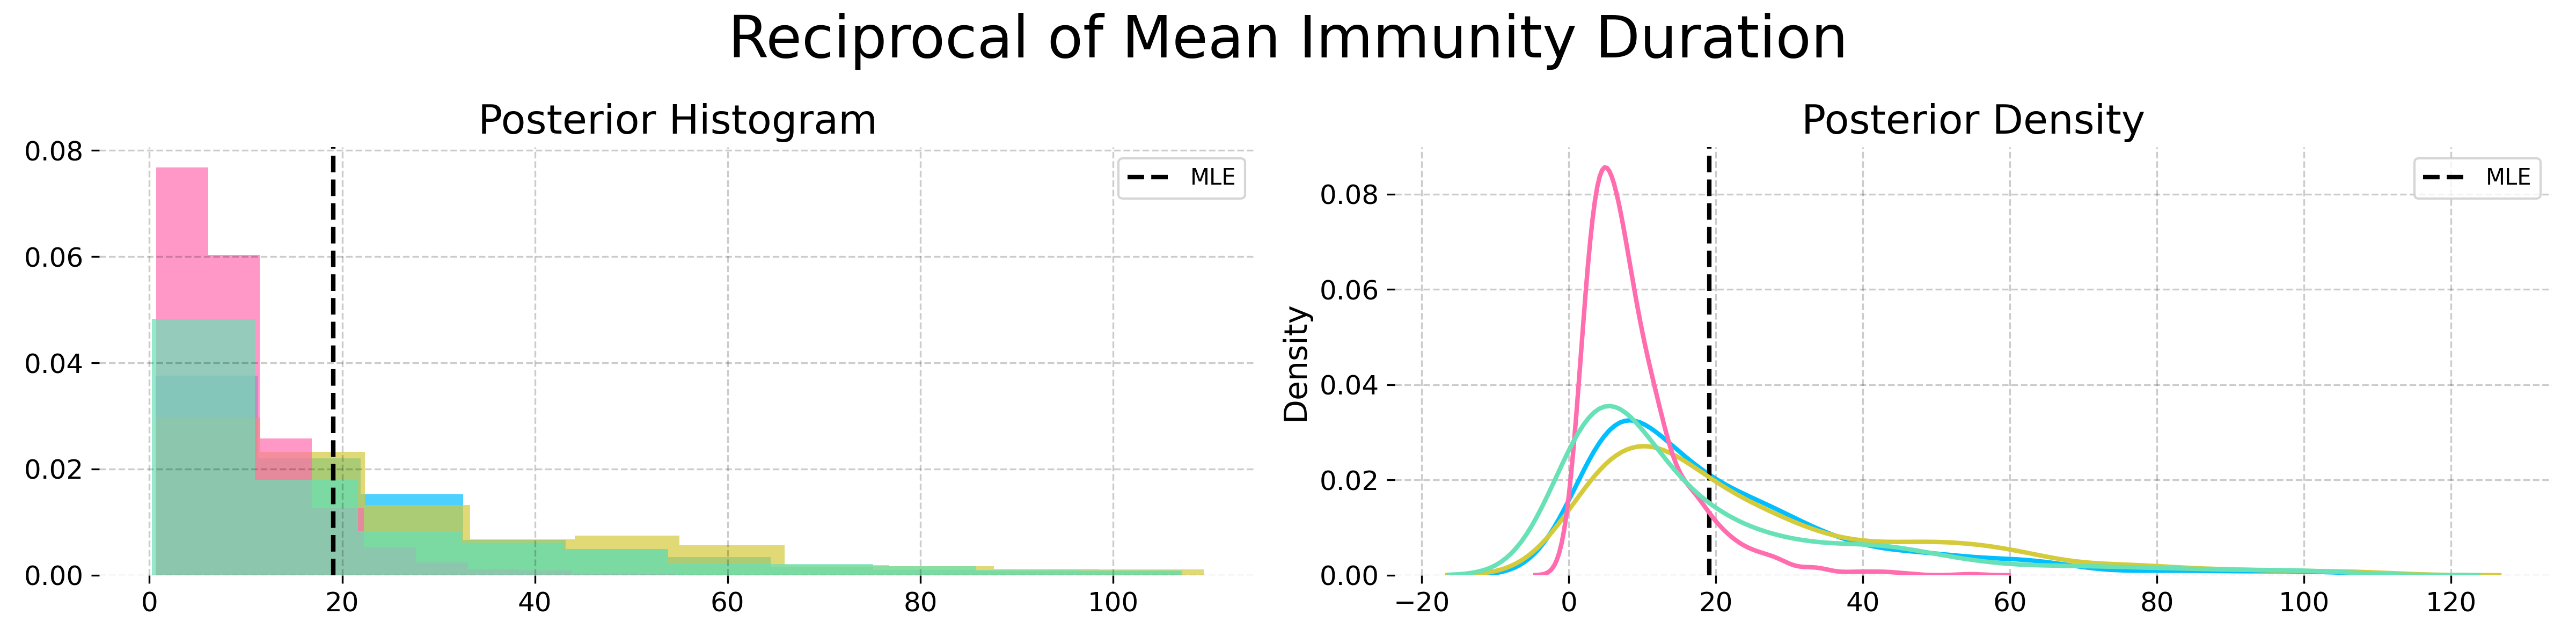
\includegraphics[scale=0.3]{imgs/pmcmc/nuts_eb/Reciprocal of Mean Immunity Duration.png}
    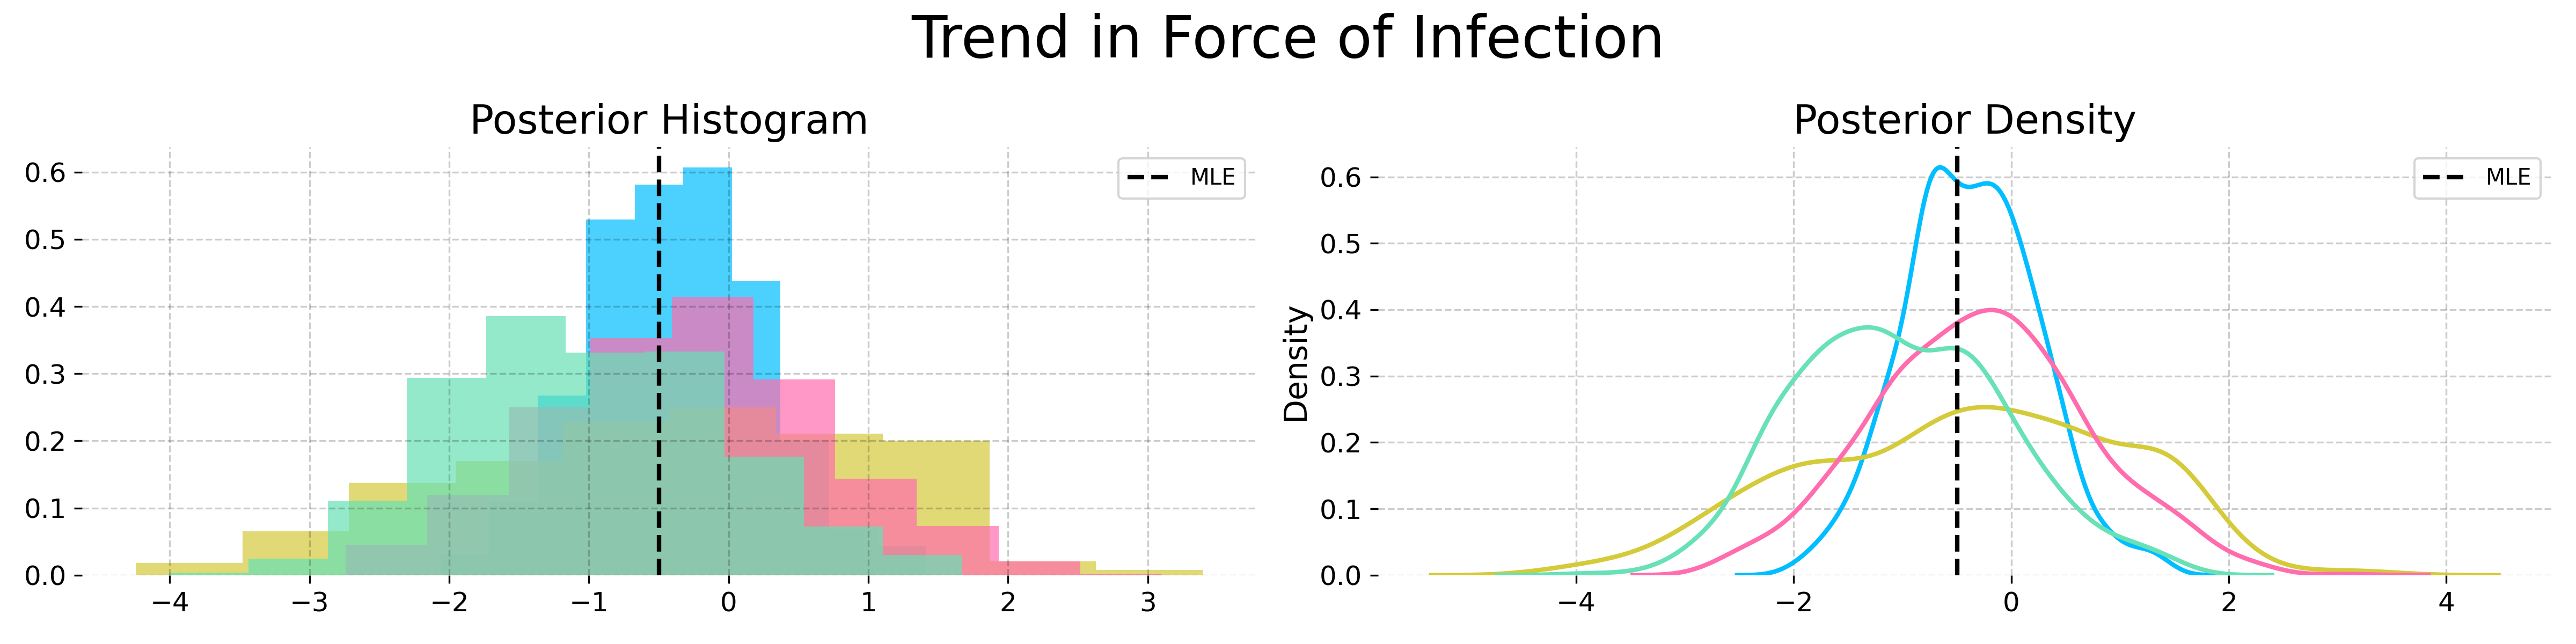
\includegraphics[scale=0.3]{imgs/pmcmc/nuts_eb/Trend in Force of Infection.png}
    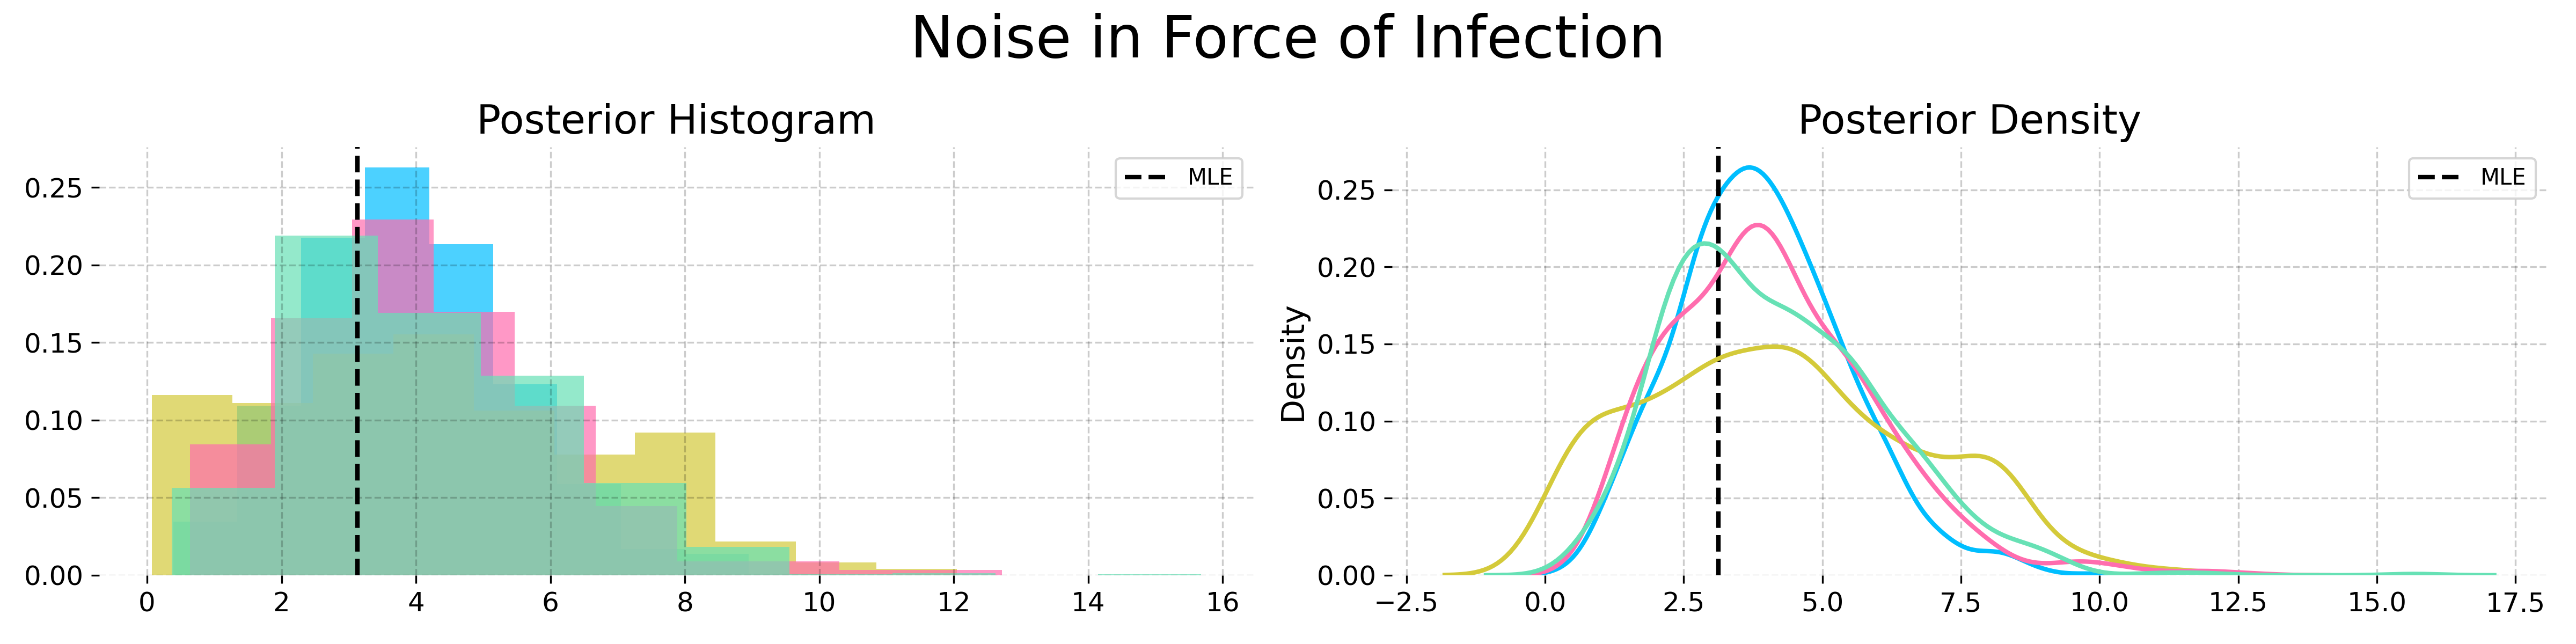
\includegraphics[scale=0.3]{imgs/pmcmc/nuts_eb/Noise in Force of Infection.png}
    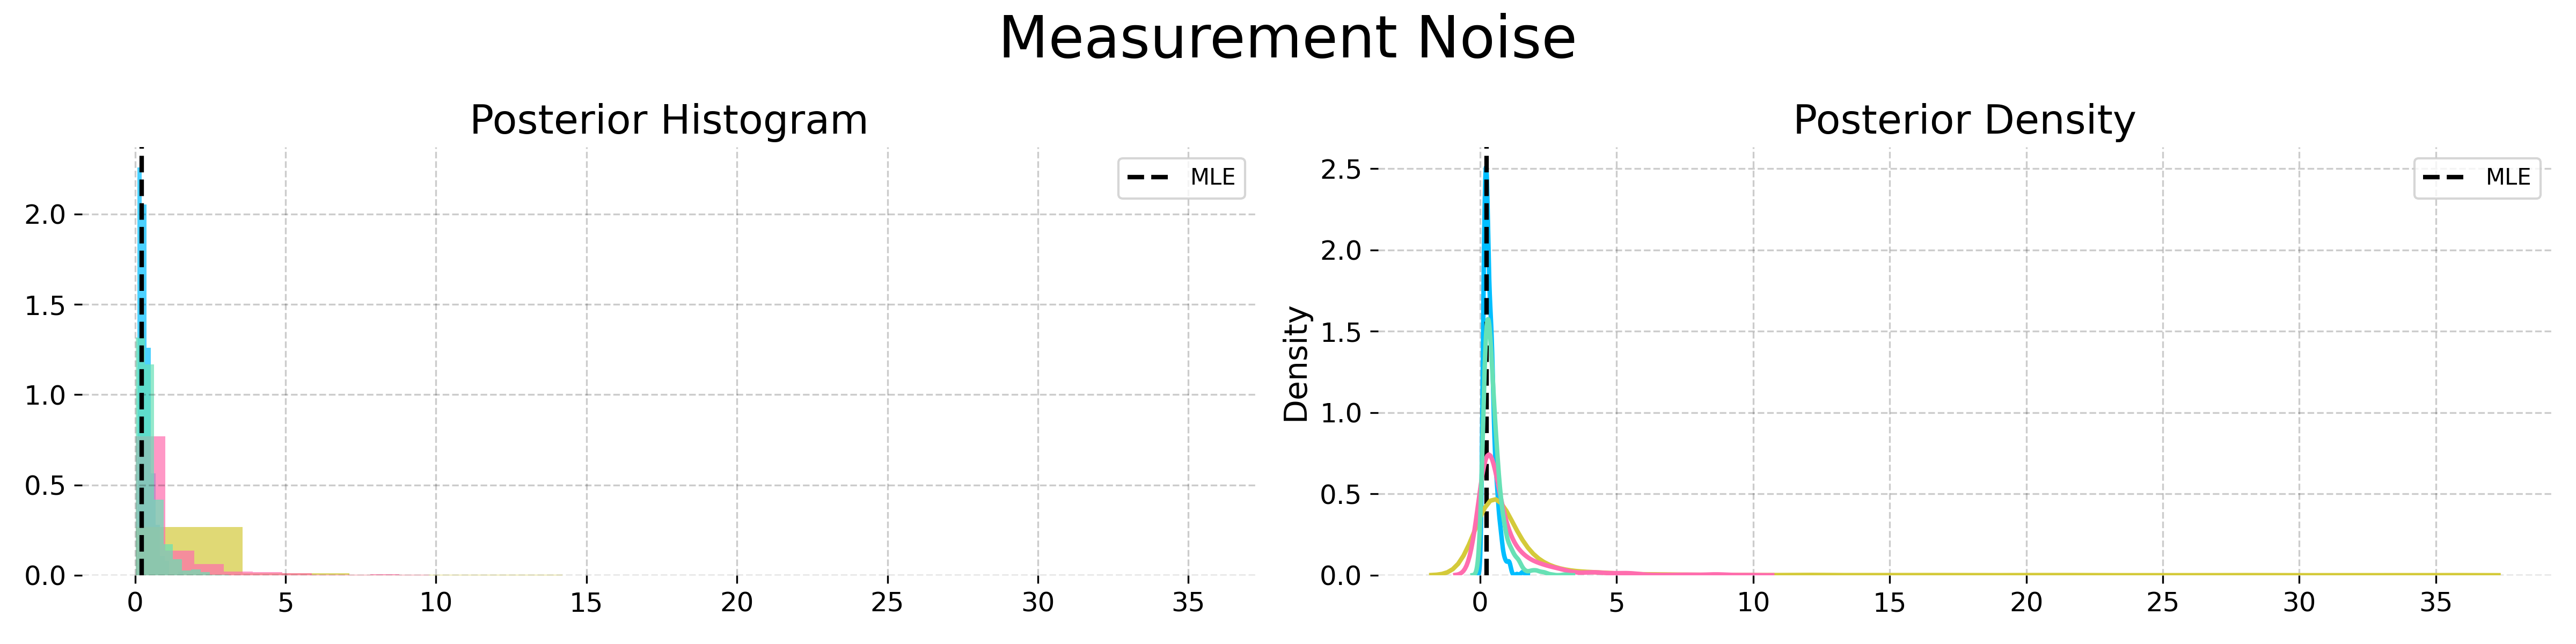
\includegraphics[scale=0.3]{imgs/pmcmc/nuts_eb/Measurement Noise.png}
    \caption{Posterior estimates from NUTS powered by MOP-$\alpha$ with the informative nonparametric empirical prior obtained from a KDE on the IF2 parameter cloud. The posterior estimates from each chain are largely in agreement.}
    \label{fig:posteriors}
\end{figure}

